\documentclass{article}

% packages
\usepackage{amsmath, amsthm, thmtools, amsfonts, amssymb, luacode, catchfile, tikzducks, hyperref, ifthen}
\ifcsname c@kobocompile\endcsname
	\usepackage[a5paper, total={1072pt, 1448pt}, margin=10pt, includeheadfoot]{geometry} % set page margins
\else
	\usepackage[a4paper, margin=50pt, includeheadfoot]{geometry}
\fi
\usepackage[shortlabels]{enumitem}
\usepackage[skip=3pt, indent=0pt]{parskip}

% language
\usepackage[bidi=basic, layout=tabular, provide=*]{babel}
\ifcsname c@english\endcsname
	\babelprovide[main, import]{english}
\else
	\babelprovide[main, import]{hebrew}
	\babelprovide{rl}
\fi
%\babelfont{rm}{Libertinus Serif}
\babelfont{rm}[Renderer=Harfbuzz]{Libertinus Serif}
\babelfont{sf}{Libertinus Sans}
\babelfont{tt}{Libertinus Mono}

% style
\AddToHook{cmd/section/before}{\clearpage}	% Add line break before section
\linespread{1.3}
\setcounter{secnumdepth}{0}		% Remove default number tags from sections, this won't do well with theorems
\AtBeginDocument{\setlength{\belowdisplayskip}{3pt}}
\AtBeginDocument{\setlength{\abovedisplayskip}{3pt}}
\graphicspath{ {../images/} }

% operators
\DeclareMathOperator\cis{cis}
\DeclareMathOperator\Sp{Sp}
\DeclareMathOperator\tr{tr}
\DeclareMathOperator\im{Im}
\DeclareMathOperator\re{Re}
\DeclareMathOperator\diag{diag}
\DeclareMathOperator*\lowlim{\underline{lim}}
\DeclareMathOperator*\uplim{\overline{lim}}
\DeclareMathOperator\rng{rng}
\DeclareMathOperator\Sym{Sym}
\DeclareMathOperator\Arg{Arg}
\DeclareMathOperator\Log{Log}
\DeclareMathOperator\dom{dom}
\DeclareMathOperator\supp{Supp}
\DeclareMathOperator\var{Var}
\DeclareMathOperator\cov{Cov}

% commands
%\renewcommand\qedsymbol{\textbf{מש''ל}}
%\renewcommand\qedsymbol{\fbox{\emoji{lizard}}}
\newcommand{\Aa}[0]{\mathcal{A}}
\newcommand{\Bb}[0]{\mathcal{B}}
\newcommand{\CC}[0]{\mathbb{C}}
\newcommand{\Cc}[0]{\mathcal{C}}
\newcommand{\EE}[0]{\mathbb{E}}
\newcommand{\FF}[0]{\mathbb{F}}
\newcommand{\Ff}[0]{\mathcal{F}}
\newcommand{\Ii}[0]{\mathcal{I}}
\newcommand{\Gg}[0]{\mathcal{G}}
\newcommand{\Ll}[0]{\mathcal{L}}
\newcommand{\Mm}[0]{\mathcal{M}}
\newcommand{\NN}[0]{\mathbb{N}}
\newcommand{\Nn}[0]{\mathcal{N}}
\newcommand{\PP}[0]{\mathbb{P}}
\newcommand{\Pp}[0]{\mathcal{P}}
\newcommand{\QQ}[0]{\mathbb{Q}}
\newcommand{\RR}[0]{\mathbb{R}}
\newcommand{\Rr}[0]{\mathcal{R}}
\newcommand{\Ss}[0]{\mathcal{S}}
\newcommand{\TT}[0]{\mathbb{T}}
\newcommand{\Uu}[0]{\mathcal{U}}
\newcommand{\Vv}[0]{\mathcal{V}}
\newcommand{\Ww}[0]{\mathcal{W}}
\newcommand{\ZZ}[0]{\mathbb{Z}}
\newcommand{\acts}[0]{\circlearrowright}
\newcommand{\explain}[2] {
	\begin{flalign*}
		 && \text{#2} && \text{#1}
	\end{flalign*}
}
\newcommand{\maketitleprint}[0]{ \begin{center}
	%\begin{tikzpicture}[scale=3]
	%	\duck[graduate=gray!20!black, tassel=red!70!black]
	%\end{tikzpicture}	
	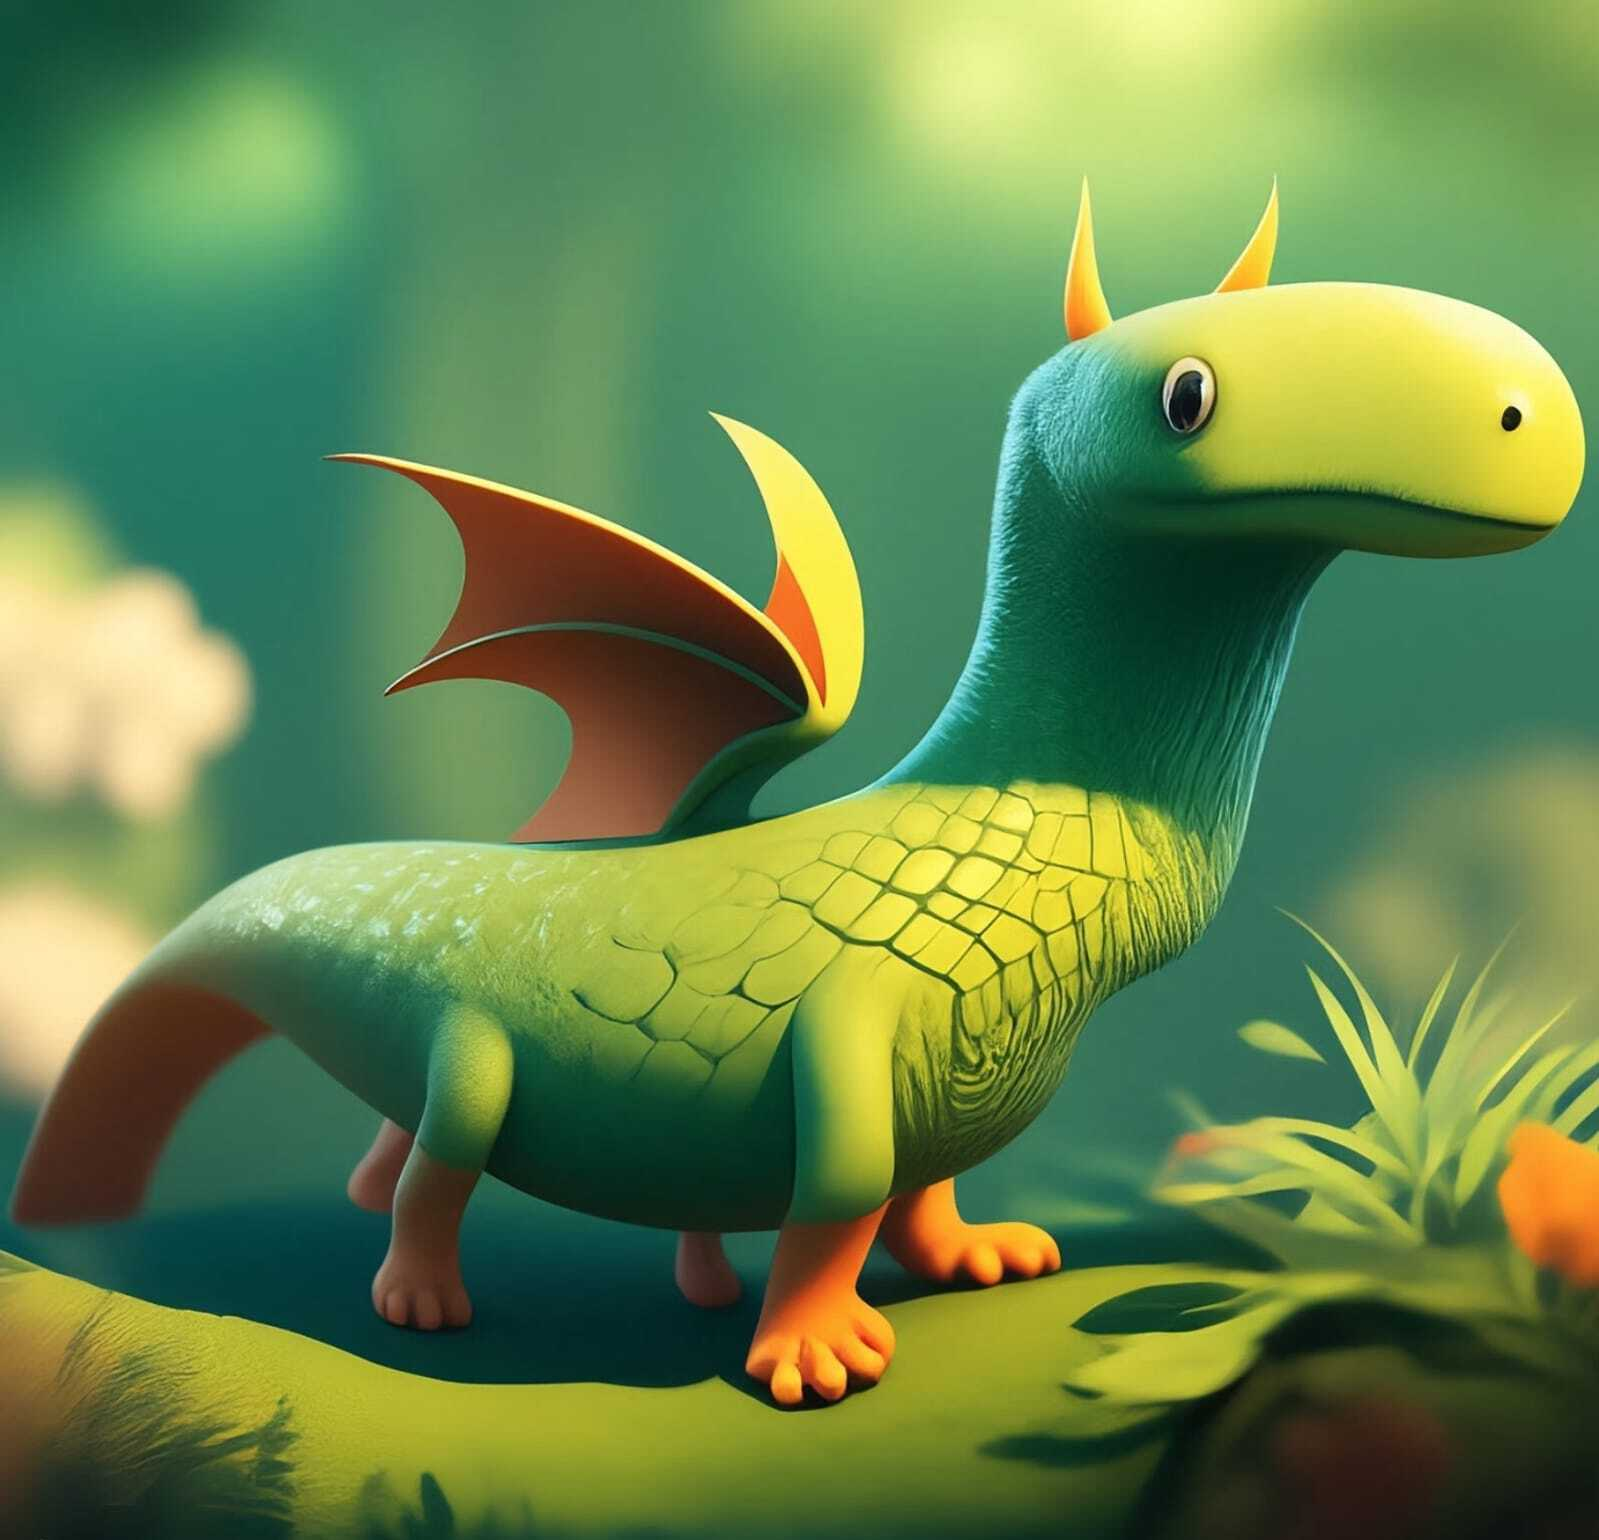
\includegraphics[width=6cm]{cover}
\end{center}
}

% theorem commands
\newtheoremstyle{c_remark}
	{}	% Space above
	{}	% Space below
	{}% Body font
	{}	% Indent amount
	{\bfseries}	% Theorem head font
	{}	% Punctuation after theorem head
	{.5em}	% Space after theorem head
	{\thmname{#1}\thmnumber{ #2}\thmnote{ \normalfont{\text{(#3)}}}}	% head content
\newtheoremstyle{c_definition}
	{3pt}	% Space above
	{3pt}	% Space below
	{}% Body font
	{}	% Indent amount
	{\bfseries}	% Theorem head font
	{}	% Punctuation after theorem head
	{.5em}	% Space after theorem head
	{\thmname{#1}\thmnumber{ #2}\thmnote{ \normalfont{\text{(#3)}}}}	% head content
\newtheoremstyle{c_plain}
	{3pt}	% Space above
	{3pt}	% Space below
	{\itshape}% Body font
	{}	% Indent amount
	{\bfseries}	% Theorem head font
	{}	% Punctuation after theorem head
	{.5em}	% Space after theorem head
	{\thmname{#1}\thmnumber{ #2}\thmnote{ \text{(#3)}}}	% head content

\ifcsname c@english\endcsname
	\theoremstyle{plain}
	\newtheorem{theorem}{Theorem}[section]
	\newtheorem{lemma}[theorem]{Lemma}
	\newtheorem{proposition}[theorem]{Proposition}
	\newtheorem*{proposition*}{Proposition}
	%\newtheorem{corollary}[theorem]{אין חלופה עברית}

	\theoremstyle{definition}
	\newtheorem{definition}[theorem]{Definition}
	\newtheorem*{definition*}{Definition}
	\newtheorem{example}{Example}[section]
	\newtheorem{exercise}{Exercise}[section]

	\theoremstyle{remark}
	\newtheorem*{remark}{Remark}
	\newtheorem*{solution}{Solution}
	\newtheorem{conclusion}[theorem]{Conclusion}
	\newtheorem{notation}[theorem]{Notation}
\else
	\theoremstyle{c_plain}
	\newtheorem{theorem}{משפט}[section]
	\newtheorem{lemma}[theorem]{למה}
	\newtheorem{proposition}[theorem]{טענה}
	\newtheorem*{proposition*}{טענה}
	%\newtheorem{corollary}[theorem]{אין חלופה עברית}

	\theoremstyle{c_definition}
	\newtheorem{definition}[theorem]{הגדרה}
	\newtheorem*{definition*}{הגדרה}
	\newtheorem{example}{דוגמה}[section]
	\newtheorem{exercise}{תרגיל}[section]

	\theoremstyle{c_remark}
	\newtheorem*{remark}{הערה}
	\newtheorem*{solution}{פתרון}
	\newtheorem{conclusion}[theorem]{מסקנה}
	\newtheorem{notation}[theorem]{סימון}
\fi

% Questions related commands
\newcounter{question}
\setcounter{question}{1}
\newcounter{sub_question}
\setcounter{sub_question}{1}

\ifcsname c@english\endcsname
	\newcommand{\question}[1][0]{
		\ifthenelse{#1 = 0}{}{\setcounter{question}{#1}}
		\section{Question \arabic{question}}
		\addtocounter{question}{1}
		\setcounter{sub_question}{1}
	}

	\newcommand{\subquestion}[1][0]{
		\ifthenelse{#1 = 0}{}{\setcounter{sub_question}{#1}}
		\subsection{Part \alph{sub_question}}
		\addtocounter{sub_question}{1}
	}
\else
	\newcommand{\question}[1][0]{
		\ifthenelse{#1 = 0}{}{\setcounter{question}{#1}}
		\section{שאלה \arabic{question}}
		\addtocounter{question}{1}
		\setcounter{sub_question}{1}
	}

	\newcommand{\subquestion}[1][0]{
		\ifthenelse{#1 = 0}{}{\setcounter{sub_question}{#1}}
		\subsection{סעיף \localecounter{letters.gershayim}{sub_question}}
		\addtocounter{sub_question}{1}
	}
\fi

% import lua and start of document
\directlua{common = require ('../common')}

\GetEnv{AUTHOR}

% headers
\author{\AUTHOR}
\date\today

\title{פתרון מטלה 04 --- מבנים אלגבריים 1 (80445)}

\begin{document}
\maketitle
\maketitleprint{}

\Question{}
\Subquestion{}
הכוונה ברורה לי אבל עוד לפני שקראתי את שאר השאלה אני רוצה אינטואיטיבית להשתמש ב־$D_n$ וצביעה מעל קבוצה.

\Subquestion{}
נגדיר $X_{n, q} = {[q]}^{[n]}$.
נוכיח שהחבורה $D_n$ משרה פעולה על הקבוצה $X_{n, q}$ על־ידי
\[
	\forall f \in X_{n, q} \forall \sigma \cdot f(k) = f(\sigma^{-1}(k))
\]
\begin{proof}
	אנו כבר יודעים כי החבורה $D_n$ היא פעולה מעל $[n]$ על־ידי $\forall g \in D_n, x \in [n] : g \cdot x = g(x)$. \\*
	בתרגול הוכחנו כי בהינתן קבוצה ופעולה עליה, ניתן להרחיב את הפעולה לצביעה של הקבוצה על־ידי
	\[
		\forall g \in D_4, f \in {[q]}^{[n]} : \forall x \in [n], g \cdot f(x) = f(g^{-1} \cdot x)
	\]
	ומצאנו כי הטענה נכונה.
\end{proof}

\Subquestion{}
נחשב את מספר המסלולים של $D_n$ על $X_{n, q}$.

נגדיר $r = (1 \dots n)$ תמורת סיבוב ו־$s(k) = n - k + 1$ פונקציית ההיפוך, לכן $D_n = \langle r, s \rangle$. \\*
תהי צביעה $f \in {[q]}^{[n]}$ כלשהי, אז נבחין כי אילו היא מורכבת מיותר צבע אחד, דהינו $\lnot \exists c : \forall k \in [n] : f(k) = c$, אז מתחייב כי $\exists n : f(n) \ne f(n + 1)$ ונוכל להסיק
\[
	Fix(f) = \{ f\} \implies |Fix(f)| = 1
\]
יהי $m \in \NN$ כך ש־$1 < m \le n$, ונבחן את $r^m$, סיבוב ב־$m$ איברים.
אילו $m \big| n$ אז קל לראות כי ישנן $q^m$ צביעות אפשריות, אילו לעומת זאת $m \nmid n$ אז נוכל להוכיח בדומה למקרה $m = 1$ שמספר הצביעות האפשרי הוא צביעה אחידה, דהינו $q$ אפשרויות.
נגדיר פונצקיה $\mu : \NN \to \NN$ המשקפת את מספר הצביעות המושרה על־ידי $r^m$ כזה, נגדירה להיות
\[
	\mu(m) = \begin{cases}
		q^m & m \mid n \\
		q & m \nmid n
	\end{cases}
\]
ואף מתקיים $Fix(r^m) = \mu(m)$ ישירות על־פי הגדרה. \\*
נבחן את המקרה השני והוא $s r^m \in D_n$ כשאר $0 \le m < n$. \\*
נשים לב כי $sr^m = {(sr^m)}^{-1}$ ולכן נובע כי $\forall k \in [n] : f(k) = f(sr^m k)$ ולמעשה נוכל להשתמש בהצמדה זו לקבוע כי ישנן $\lfloor \frac{n}{2} \rfloor q$ צביעות. \\*
נסכם:
ב־$\langle r, s \rangle$ ישנם $2n$ איברים בדיוק, כולם מהצורה $r^m$ או $s r^m$ עבור $0 \le m < n$. נבנה פונקציה $\nu : D_n \to \NN$ המייצגת את כמות הצביעות על־פי פעולה מהחבורה:
\[
	Fix(s^l r^m) = \nu(s^l r^m) = \begin{cases}
		q \lfloor \frac{n}{2} \rfloor & l = 1 \\
		\mu(m) & l = 0
	\end{cases}
\]
ונשתמש בלמה של ברנסייד לקבל כי מספר המסלולים מוגדר על־ידי
\[
	|X_{n, q} / D_n| = \frac{1}{|D_n|} \sum_{s^l r^m \in D_n, l \in \{0, 1\}, 0 \le m < n} \nu(s^l r^m)
	= \frac{1}{|D_n|} \sum_{s^l r^m \in D_n, l \in \{0, 1\}, 0 \le m < n} \begin{cases}
		q \lfloor \frac{n}{2} \rfloor & l = 1 \\
		q^m & l = 0, m \mid n \\
		q & l = 0, m \nmid n
	\end{cases}
\]

\Subquestion{}
נחשב את מספר המסלולים שמשרה $\langle r \rangle$ על $X_{n, q}$.

למעשה כבר חישבנו מספר זה בדיוק וקיבלנו כי הוא
\[
	|X_{n, q} / \langle r \rangle |
	= \frac{1}{|D_n|} \sum_{0 \le m < n} \begin{cases}
		q^m & m \mid n \\
		q & m \nmid n
	\end{cases}
\]

\Question{}
\Subquestion{}
יהיו $v_0, \dots, v_3$ קודקודי $\Delta^3$ ויהיו $E = \left\{ \{v_i, v_j\} \middle| i \ne j \right\}$ קבוצת הקשתות של $\Delta^3$.
נוכיח ש־$\Sym_+(\Delta^3)$ פועלת על הקבוצה $E$. 
\begin{proof}
	בתרגול מצאנו כי $\Sym_+(\Delta^3)$ היא פעולה על $\Delta^3$ עצמה. \\*
	נגדיר $\cdot : \Sym_+(\Delta^3) \times E \to E$ על־ידי $g \cdot \{v_i, v_j\} = \{g \cdot v_i, g \cdot v_j\}$.
	עתה נבדוק אם התכונות של פעולה מתקיימות:
	\begin{itemize}
		\item נייטרליות: $\forall k \in E, e \cdot k = \{ e \cdot v_i, e \cdot v_j \} = \{v_i, v_j \} = k$.
		\item $\forall g, h \in \Sym_+(\Delta^3), x \in E: h \cdot (g \cdot x): h \cdot \{g v_i, g v_j \} = \{ (hg) v_i, (hg)v_j\} = (hg) \cdot x$.
	\end{itemize}
	ומצאנו כי התכונות נשמרות וזוהי פעולה.
\end{proof}

\Subquestion{}
יהי $m \in \NN$ ונסמן $X = {[m]}^E$ הצביעה של $E$ ב־$m$ צבעים.
נראה כי החבורה $\Sym_+(\Delta^3)$ פועלת על הקבוצה $X$ על־ידי $\forall T \in X, f \in X : T \cdot f(x) = f(T^{-1} \cdot x)$.
\begin{proof}
	למעשה, על־ידי שימוש בסעיף הקודם וטענה מהתרגול נקבל ישירות כי זוהי אכן פעולה מוגדרת.
\end{proof}

\Subquestion{}
נמצא את מספר המסלולים של הפעולה $\Sym_+(\Delta^3)$ על $X$.

בתרגול מצאנו כי החבורה מורכבת מאוסף המחזורים מגודל $3$ ומהרכבה של מחזורים זרים בגודל $2$, ובסך הכול יש $12$ איברים בחבורה.\\*
עבור העתקת הזהות נוכל לצבוע כל צלע בצביעה נפרדת, ונקבל כי יש $m^6$ צביעות כמספר הצלעות בטטרההדרון. \\*
עבור מחזור בגודל שלוש נקבל שאנו מסובבים שלוש צלעות ובשאר אין שינוי, ולכן נוכל לצבוע את שלוש הצלעות בצבע אחד ואת שלוש הצלעות האחרות בצבע נפרד כל אחת, ונקבל $m^4$ צביעות. \\*
עבור שני מחזורי $2$ אנו מסובבים שתי צלעות סביב עצמן ובעצם לא משפיעים עליהן בפעולה, ואת ארבע הצלעות האחרות אנו מסובבים ומחליפים אותן בזוגות, לכן נוכל לצבוע את שתי הצלעות במחזורים בנפרד ושני זוגות צלעות בנפרד, ונקבל $m^4$ צביעות. \\*
לכן מהלמה של ברנסייד נקבל
\[
	|X/E| = \frac{m^6 + 11m^4}{12}
\]
דהינו מספר המסלולים השונים הוא $\frac{m^6 + 11m^4}{12}$.

\Question{}
\Subquestion{}
תהי חבורה $G$ ויהי $N \le G$ תת־חבורה, נוכיח שהתנאים הבאים שקולים:
\begin{enumerate}
	\item $N$ נורמלית.
	\item $\forall g \in G : g^{-1} N g \le N$.
	\item $\forall g \in G : gN = Ng$.
\end{enumerate}
\begin{proof}
	\begin{itemize}
		\item $1 \to 2$: \\*
			תהי $N$ תת־חבורה נורמלית של $G$.
			ההגדרה גורסת כי $\forall g \in G : gNg^{-1} = N$, לכן נוכל להסיק בפרט גם $\forall g \in G : g^{-1} N g \le N$, שכן כל חבורה מהווה תת־חבורה לעצמה.
		\item $2 \to 3$: \\*
			נניח כי $\forall g \in G : g^{-1} N g \le N$.
			נכפיל משמאל ונקבל $N g \le g N$, אם נבחר את $g^{-1}$ נקבל גם $g N g^{-1} \le N$ ומכאן נסיק $g N \le N g$, ובסך הכול $g N = Ng$.
		\item $3 \to 1$: \\*
			נניח כי $\forall g \in G : g N = N g$.
			לכן גם $g N g^{-1} = N g g^{-1} = N$ וקיבלנו כי $N \trianglelefteq G$.
	\end{itemize}
\end{proof}

\Subquestion{}
נוכיח שאם $N \le G$ וגם $[G : N] = 2$ אז $N \trianglelefteq G$.
\begin{proof}
	נתון כי האינדקס של המחלקות של $N$ ב־$G$ הוא $2$. \\*
	קיימות אם כן שתי מחלקות בלבד, והן $N, gN$ עבור $g \in G$ כלשהו. \\*
	מהתכונות של מחלקות נובע ש־$g N = N$ אם ורק אם $g \in N$, לכן נניח $g \notin N$ ונקבל $N \ne gN$ שתי המחלקות היחידות. \\*
	באופן דומה עבור אותו $g$ נקבל $N \ne N g$, אבל ידוע כי יש רק שתי מחלקות ויש התאמה בין מחלקות ימניות ושמאליות ולכן נסיק $g N = N g$, ומהסעיף הקודם נסיק $N \trianglelefteq G$.
\end{proof}

\Subquestion{}
תהי חבורה $G$, ונוכיח ש־$Z(G) \trianglelefteq G$.
\begin{proof}
	יהי $h \in G$, נבחין כי $h Z(G) = \{ hx \mid \forall g \in G : gx = xg\} = \{ xh \mid \forall g \in G: xg = gx \} = Z(G) h$.
	נסיק אם כן מסעיף א' ש־$Z(G) \trianglelefteq G$.
\end{proof}

\Question{}
תהי חבורה $G$ ונסמן $X = \{ H \subset G \mid H \le G \}$.

\Subquestion{}
נוכיח שהפעולה $\cdot : G \times X \to X$ המוגדרת על־ידי $g \cdot H = gHg^{-1}$ היא פעולה של $G$ על $X$.
\begin{proof}
	נבחין תחילה כי האיבר הנייטרלי משמר את הקבוצה:
	\[
		\forall H \in X : e_G H e_G^{-1} = H
	\]
	נבחין גם כי תכונת השימור המגדירה פעולות על קבוצות חלה:
	\[
		\forall H \in X, g, h \in G: g \cdot (h \cdot H) = g \cdot (hHh^{-1}) = gh H h^{-1} g^{-1} = (gh) H {(gh)}^{-1} = (gh) \cdot H
	\]
	ומצאנו כי $G$ היא אכן פעולה מעל $X$.
\end{proof}

\Subquestion{}
נבחין במייצב:
\[
	N_G(H) = Stab(H) = \{ g \in G \mid g H g^{-1} = H \}
\]
ונוכיח כי $H \trianglelefteq N_G(H)$.
\begin{proof}
	יהי $h \in H$, אז כמובן נובע $h \in N_G(H)$ שכן $e h e^{-1} = h$.
	עוד נשים לב כי $forall g \in N_G(H) : g H g^{-1} = H$ וזוהי למעשהה ישירות הגדרת תת־חבורה נורמלית ונובע $H \trianglelefteq N_G(H)$.
\end{proof}

\Subquestion{}
נוכיח כי לכל $H \in X$ מתקיים $C_G(H) \trianglelefteq N_G(H)$, דהינו המרכז של תת־חבורה הוא תת־חבורה נורמלית של המייצב של תת־הקבוצה.
\begin{proof}
	נבחין כי $C_G(H) \le H \le N_G(H)$ ולכן $g \in C_G(H) \iff \forall h \in H : g h g^{-1} = h \implies g H g^{-1} = H$
	\[
		C_G(H) \trianglelefteq N_G(H)
		\iff
		\forall g \in C_G(H) : g C_G(H) g^{-1} = C_G(H)
		\iff
		\forall g \in C_G(H), h \in N_G(H) : g h g^{-1} = h
	\]
	ומצאנו כי ההגדרות של שתי הקבוצות משרות נורמליות ומתקיים $C_G(H) \trianglelefteq N_G(H)$.
\end{proof}

\Subquestion{}
נמצא דוגמה כך ש־$C_G(H) \ne N_G(H)$.

נבחן את $G = D_4, H = \langle  \sigma \rangle$. \\*
נראה כי $\forall \sigma^m \in H : \sigma \sigma^m \sigma^3 = \sigma^m$ ולכן $\sigma \in C_G(H)$.
לעומת זאת $\tau \sigma \tau^{-1} = \sigma^3 \ne \sigma$ ולכן $\tau \notin C_G(H)$. \\*
בסך הכול $C_G(H) = \langle \sigma \rangle = H$. \\*
בתהליך זה מצאנו כי $\sigma H \sigma^3 = H$ וגם $\tau H \tau = H$ ולכן $N_G(H) = G$ ומצאנו $C_G(H) \ne N_G(H)$.

\Question{}
יהי $Q = \{ \pm 1, \pm i, \pm j, \pm k\}$ ומוגדר $i^2 = j^2 = k^2 = ijk = -1$ וגם $\forall x \in Q: (-1) x = x (-1) = -x$. נתון כי זוהי חבורה.

\Subquestion{}
נוכיח כי $Q$ לא אבלית.
\begin{proof}
	נניח בשלילה כי היא אבלית. \\*
	אנו יודעים כי $ij = {(j^{-1} i^{-1})}^{-1} = -(j (-1)(-1) i) = -ji$ בבתירה לטענה כי $ij = ji$ ולכן $Q$ לא אבלית.
\end{proof}

\Subquestion{}
נראה כי $Q$ לא איזומורפית ל־$D_4$.

אילו ננסה לבנות הומומורפיזם בין החבורות, נקבל כי $\varphi(i^2) = \varphi(i) \varphi(i) = \varphi(-1)$
וגם $\varphi(-1) = \varphi(j) \varphi(j)$ אבל לא נוכל למצוא שני איברים שונים ב־$D_4$ שהרכבתם בעצמם היא זהה אך שאיננה האיבר הנייטרלי.

\Subquestion{}
נחשב את $Z(Q)$.

נשים לב כי ישנם שמונה איברים יחודיים ב־$Q$. \\*
כמובן $1$ נייטרלי לסדר ההכפלה, ועל־פי הגדרה גם $-1$. \\*
לעומת זאת מצאנו כי $ij = -ji, ik = -ki, jk = -kj$ ולכן נוכל להסיק כי איברים אלה לא משמרים נייטרליות. \\*
לכן $Z(Q) = \{1, -1\}$.

\Subquestion{}
נמצא את כל תת־החבורות של $Q$ ונבדוק אילו מהן נורמליות.

נבחין כי $i^{-1} = -i$ אבל $ij = k$ ולכן $\langle i, j \rangle = \langle i, j, k \rangle = Q$. \\*
נסיק כי כל תת־החבורות הן $\{ \{1, -1\}, \langle i \rangle, \langle j \rangle, \langle k \rangle , Q\}$. \\*
נראה כי $i (-1) (-i) = -1$ וממעבר דומה נוכל להסיק כי $\{1, -1\}$ היא נורמלית. \\*
עבור $\langle i \rangle$ נבחן את $j i (-j) = -j k = -i$ וממעבר דומה על $k$ נקבל כי גם $\langle i \rangle$ נורמלית. \\*
מכאן נסיק ישירות כי כל תת־החבורות של $Q$ הן נורמליות.

\Subquestion{}
נמצא את מחלקות הצמידות של $Q$.

מצאנו כי כל תת־קבוצה היא נורמלית ולכן גם צמודה לעצמה בלבד, ונסיק כי יש ארבע מחלקות צמידות.

\end{document}
